\documentclass{csfourzero}

\title{The Shortest Path Problem: 
Impact of Varying Properties on Uninformed Algorithms}
\author{Pontus Henningsson}
\date{\today}
% A useful package to support on-line references
\usepackage{url}
\usepackage{natbib}
\usepackage{graphicx}
\graphicspath{ {./images/} }

\bibliographystyle{plain}
\abstract{Pathfinding is widely used in our everyday lives, from finding the fastest way home to network routing. This paper compares three common uninformed algorithms on the metrics running time and accuracy when solving the shortest path problem on a grid-based weighted undirected graph with varying properties of the graph. The results finds that Dijkstra’s is the most efficient algorithm out of the three being compared in regards to the metrics run time and accuracy. The tests shows a slight increase on the performance of the algorithms on run time on a graph with greater complexity and longer edges, with the exception of DFS in terms of run time on longer edges on a graph with greater complexity.}


\begin{document}
\maketitle


\section{Introduction}
\label{sec:intro}
Pathfinding is used frequently in our everyday lives and the route wanted is more often than not the shortest route, for instance finding the shortest route home from work. "The shortest path problem" concerns itself with finding the shortest path possible between two nodes (or vertices) in a graph \cite{rachmawati2020analysis}. 


To solve the shortest path problem, pathfinding algorithms have been developed and researched. Common algorithms include among others Depth-First Search (DFS) \cite{reif1985depth}, Breadth-First Search (BFS) \cite{5219222}, Dijkstra's algorithm \cite{dijkstra1959} and A* \cite{4082128}. The different algorithms have their own strengths and weaknesses depending on the situation \cite{ashish2021path}. A practical application of using a graph is when applied to a geographical map, where the nodes represents locations, such as a cities, and the edges represents the roads that connects to the cities \cite{monzonis2019pathfinding}. Pathfinding algorithms can be divided into two different categorizes: informed and uninformed. Informed algorithms, such as A*, use heuristic functions to find the shortest path possible by prioritizing cheaper nodes. Uninformed algorithms on the other hand conduct a brute-force search (also called blind search) where the algorithm traverses the entire graph to find the shortest path possible. The main benefit of the informed algorithms is that they are faster and cheaper to execute, but cannot always guarantee that the shortest path is found. Uninformed algorithms, except DFS, guarantee that the shortest path is found with the cost of added computing time and memory usage \cite{ashish2021path}.


As technology becomes a more central part of our lives, so does the need for pathfinding and thus efficient pathfinding algorithms. To keep up with the increasing demand of pathfinding, current and new pathfinding algorithms need to be as efficient as possible \cite{foead2021systematic}. There might be times however when there needs to be a guarantee that the algorithm finds the shortest path, making uninformed algorithms useful. Uninformed algorithms can also be applied to a multitude of problems as it does not take the target problem into account and finds the target using a brute-force approach \cite{ashish2021path}.


This paper sets out to compare three uninformed pathfinding algorithms: BFS, DFS and Dijkstra's. The data used will consists of four different graphs with variying properties on a grid-based map with European cities and the travelling connections between them. The algorithms performance will be compared from the metrics running time and accuracy when trying to solve the shortest path problem on a graph with varying properties. 

\vspace{1cm} 

\section{Background and Related Work}
\label{sec:lit}
Research has been conducted on the comparison of different pathfinding algorithms in relation to travelling, such as the research paper \cite{4631975} published in 2008 by Chiong et al. The study suggests that informed algorithms generally perform better than uninformed, although Dijkstra's and modifications to it can serve as a feasible application for efficient pathfinding. Four different tests were run with varying complexity of the graph in regards to the amount of nodes: 8, 15, 75 and 100 nodes. What the paper does not evaluate is how the distance between the nodes (the length of the edges) impacts the algorithms performance. In the paper uninformed algorithms perform worse as the graph gets more complex \cite{4631975}. As graphs have varying properties, such as the number of nodes or length of the edges, an algorithm that performs well in graphs with both low and high number of nodes could perform inadequately on graphs that have long edges, making it interesting to research properties other than the amount of nodes. 

Research conducted by S. Munjal et al \cite{ashish2021path} compares five common pathfinding algorithms: Dijkastra's, A*, Greedy Best First Search, BFS and DFS. The comparison is based around three criteria: complexity, reliability and if the graph is weighted or unweighted. The conclusion drawn is that the best algorithm depends on the circumstances in which it is used. This research paper does not explain what methods they have used and in what context. It is therefore unknown on what the algorithms have been applied to, such as on a geographical map, the number of nodes and edges, the distance between them and so on \cite{ashish2021path}. 

In the paper \cite{rachmawati2020analysis} by Rachmawati and Gustin, Dijkstra's and A* are compared when trying to solve the shortest path problem. The algorithms are applied to a regional scale map and a larger scale map. The algorithms are tested on their running time and their loop count when trying to find the shortest path possible. The conclusion drawn is that the two algorithms are essentially equally as efficient when used on a regional scale map, but on a larger scale map A* provides the solution faster than Dijkstra's algorithm.  However, the test is only applied to a single uninformed algorithm, Dijkstra's. To find out which uninformed algorithm is the most efficient in this pathfinding context further testing needs to be made, such as including more uninformed algorithms in the testing and varying the properties of the graph further, something which the paper does not explore \cite{rachmawati2020analysis}. 

Pathfinding algorithms is a widely researched area, and as seen by the papers previously mentioned , there is related work on comparisons of different pathfinding algorithms. Pathfinding benchmarks have been proposed \cite{6194296}. However, the metrics being evaluated, the type of graph and the tests being run are inconsistent between different research papers, making it hard to compare results of different papers.

\section{Research Questions}
\label{sec:rq}
Dijkstra's uses a starting node to a target node in a graph to find the shortest path by traversing the entire graph. The shortest path is created by connecting the starting node to all other nodes finding the shortest path to the target node. Dijkstra's guarantees that the shortest path possible is found. The downside of Dijkstra's is that it cannot use negative edges, making it limited in practice, as well as it is very slow since it traverses the entire graph to find the shortest path between the starting and target node \cite{ashish2021path}. The original Dijkstra algorithm used an array \cite{dijkstra1959} instead of a with minimum priority queue. The Dijkstra algorithm implementation in this program will use a heap with minimum priority queue. 


DFS starts at the root node and traverses the graph using an adjacency list. When visiting node v, the search is then carried on to the first unvisited node in the adjacency list. If no node exists, that search is exhausted at node v, and the search continues on the last unexhausted node visited before v until all nodes have been visited and thus exhausted \cite{reif1985depth}. DFS can get stuck in loops unable to find a solution and thus cannot guarantee that the shortest path possible is found but consumes less memory space \cite{ashish2021path}. 


Where DFS traverses the graph at depth, BFS traverses the graph at breadth. Meaning, the algorithm starts at the root node and explores all nodes at that level, then moving onto to the next depth level and exploring all nodes on that level of depth before going to the next depth level before the shortest path has been found. BFS is an uninformed algorithm just like the other algorithms used in this paper, meaning that the algorithm traverses the entire graph before finding the solution. 
BFS guarantees the shortest path but consumes more memory since all connected nodes must be stored in memory \cite{ashish2021path}. 

The algorithms performance will be recorded from the metrics running time and accuracy. Running time being measured in nanoseconds and meaning how long it takes for the algorithm to find the shortest path possible. Accuracy meaning how accurate the algorithm is when finding a path from the start to the target node: in this case if the algorithm finds the shortest path possible or not. The paper concerns itself with varying properties of a graph and will focus on exploring two of them: the distance between the nodes (the length of the edges) as well as the complexity of the graph (the amount of nodes and length of the edges). 

\vspace{0.25cm} 
The research questions are therefore as follows: 
\begin{itemize}
    \item How does distance impact the performance of the three algorithms?
    \item How does the complexity of the graph impact the performance of the three algorithms?
\end{itemize}

\vspace{0.5cm} 

\section{Experimental Design}
\label{sec:exp}
The following null hypothesis were constructed:
\begin{itemize}
    \item Dijkstra's does not perform significantly better than the other algorithms in regards to the metrics running time and and accuracy
    \item The amount of nodes will not affect the algorithms performance to a greater degree than the length of the edges will  
\end{itemize}

The alternative hypothesis being: 
\begin{itemize}
    \item Dijkstra's is the most efficient algorithm out of the three being compared in regards to the metrics running time and accuracy
    \item The amount of nodes will impact the algorithms performance more than the length of the edges will
\end{itemize}

The algorithms were implemented in a simple travelling program consisting of a graph that represents a network of places that represents nodes and connections that represents the edges through a grid-based map. The places have a few connections to places which are linked together through an adjacency list. The graph is weighted as to give the connections a numerical value, in this case a numerical value of time. For instance, going from Dublin to Stockholm takes 2 hours and 40 minutes. All weights are given in minutes which is also represents the distance. The longer the path takes in minutes, the further away the two connected places are to each other. No weights have negative values. The graph is also undirected, meaning that the connection between two places is bidirectional and the connection is the same. The graph is a simple weighted undirected graph. 


T The first program will have 10 European cities with various connections between them, the second program will have 40 European cities with various connections between them. This is tested to compare the algorithms performance in regards to the complexity of the graph. The impact of the distance in time between the places will also be tested to see if the algorithms differ in performance in regards to the length of the edges. To do this, each graph will be tested twice. The graph with 10 cities will be tested with short edges, and then tested again with long edges to compare the difference in performance when the edges are a different length. The same will be done on the graph with 40 cities. The data used is thus the nodes that represent the European cities and the edges that represent the connections between the different cities. All graphs have the same amount of edges to make the tests as equal as possible. 


All tests will be run five times for each algorithm to get accurate test results. These test results will then be analyzed and the average test result for each algorithm for every test situation (the graph with 10 cities and small edges for example) will then be presented. For every test there are independent and dependent variables. The independent variables, the inputs, are: the different graphs and their edges and nodes and the algorithms used. By inputting the aforementioned independent variables the dependent variables output are thus: accuracy, run time, loop count and the distance in time. 


All tests will be run on a MacBook Air M2 (2022) with 16GB of RAM using Java JDK 15 and JavaFX 12 in Intellij IDEA version 2022.2.3. To make the tests as accurate as possible, no other applications besides the ones required for the testing will be used or open at the same time as the tests are run. 


\section{Results}
\label{sec:results}
\vspace{0.5cm} 

\subsection{Dijkstra's does not perform significantly better than the other algorithms in regards to the metrics running time and accuracy}
\ref{tab:algorithmavg}
\ref{fig:bfsdfsdijk}
In table two the algorithm average performance on all tests combined is presented: 
%Nedanstående tabell är bra för att visa hur Dijkstras är mest effektiv och besvarar således första hypotesen. 
\begin{table}[h]
\centering
% To place a caption above a table
\caption{Algorithm averages on all tests combined}
\begin{tabular}{ |c|c|c|c| }  
 \hline 
 Algorithm & BFS & DFS & Dijkstra's  \\ 
 \hline
Accuracy* \% & 100 & 50 & 100\\ 
  \hline
  Loop Count & 23 & 23.5 & 25 \\ 
 \hline
 Run time (in nanoseconds) & 715 069 & 1 742 050 &  59 449\\ 
 \hline
 Distance** (in minutes)* & 155 & 381 & 155 \\ 
 \hline
\end{tabular}
\label{tab:algorithmavg}
\end{table}
 *Accuracy in the table meaning the percentage that the algorithm found the shortest possible. **Distance being the average distance the algorithm travels to find a path from the start to target node. Dijkstra's has a significantly lower run time than both BFS and DFS, but having a higher loop count than the two algorithms.  


Figure \ref{fig:bfsdfsdijk} displays the algorithm averages on all test for a graphical overview: 
\begin{figure}[h]
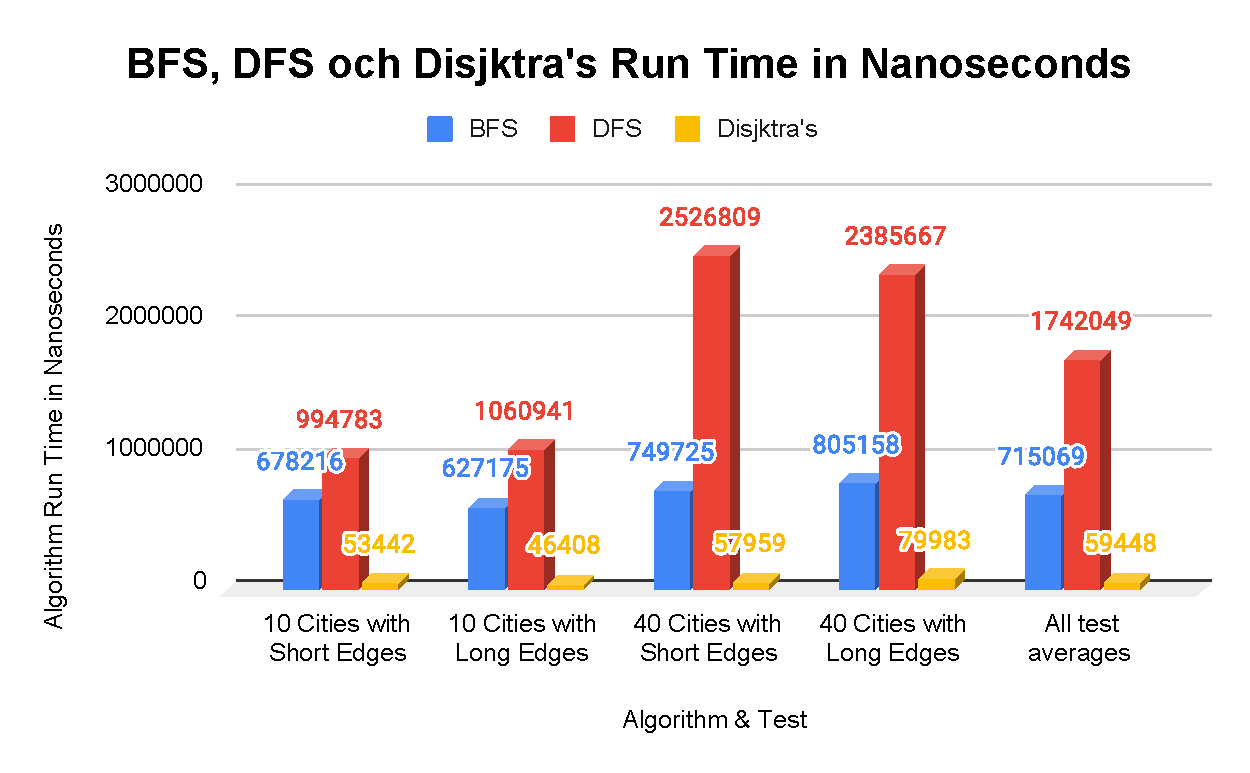
\includegraphics [scale = 0.7]{images/BFS_DFS_Dijkstra.pdf}
\caption{Algorithm run time averages }
\label{fig:bfsdfsdijk}
\end{figure}
Analyzing the results in figure \ref{fig:bfsdfsdijk}, as well as in table \ref{tab:algorithmavg}, Dijkstra's has a significantly lower run time than both BFS and DFS as well as a 100\% accuracy rate, meaning that the null hypothesis can be rejected. To affirm this, T-tests were conducted on the averages of the test, with the following results: P-value for run time averages for BFS and DFS: 1.2\%. P-value for algorithm run time averages for BFS and Dijkstra's: 0.0006\%. P-value for algorithm run time averages for DFS and Dijkstra's: 0.3\%. All of the above P-values are below 5\%, the BFS and Dijkstra's P-value and DFS and Dijkstra's significantly so, leading that the tests are statistically significant. This means that the null hypothesis can be rejected, and the alternative hypothesis can be accepted, Dijkstra's performs better than the other algorithms in regards to the given metrics. 

\vspace{1cm} 


\subsection{The amount of nodes will not affect the algorithms performance to a greater degree than the length of the edges will}
To test this null hypothesis two different tests were conducted. One where the impact of the amount of the nodes in the graph are tested, and the second testing the impact of the length of the edges. 
\ref{fig:avgdifnode}
\ref{tab:pvaluevar}

Test results from testing the impact of the amount of the nodes as well as the length of the edges in the graph in regards to the algorithms performance are displayed in the figure \ref{fig:avgdifnode}.
\begin{figure}[h]
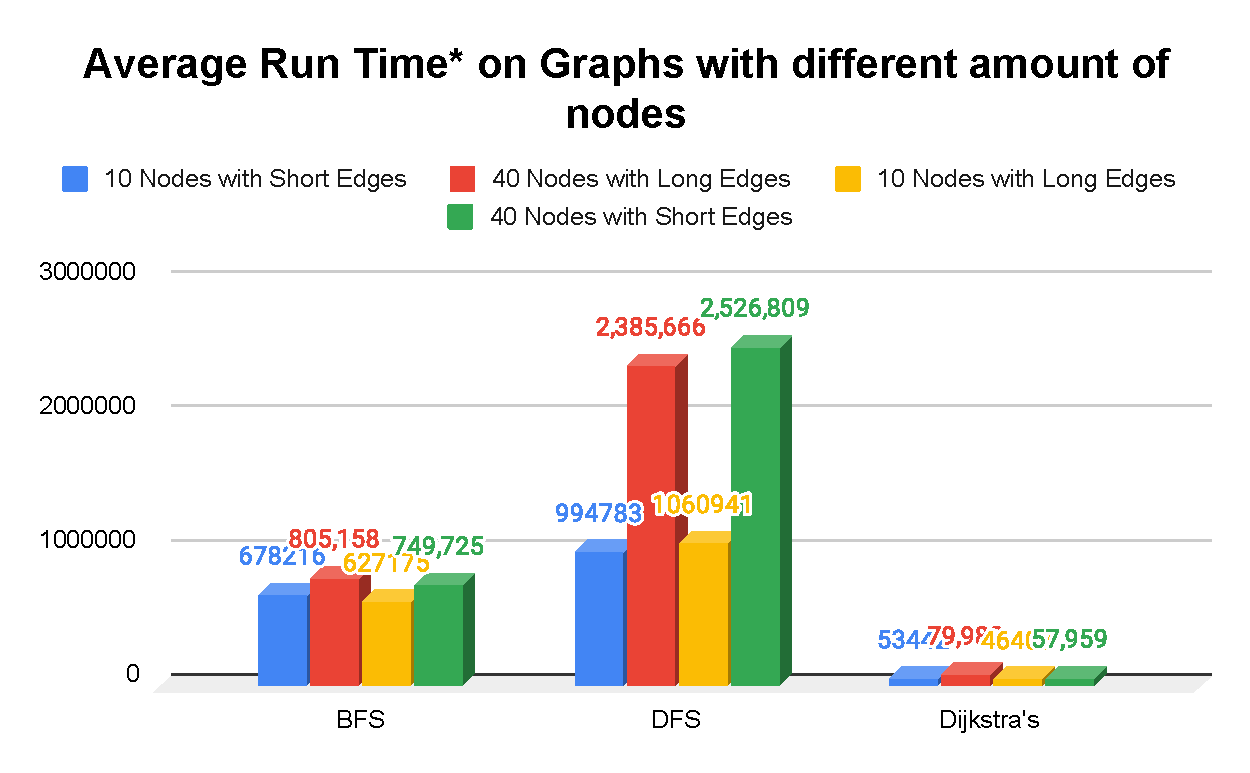
\includegraphics [scale = 0.7]{images/AVG_RUNTIME_DIF_NODES.pdf}
\caption{Algorithm run time averages }
\label{fig:avgdifnode}
\end{figure}

Run time is higher on graphs with more nodes for all algorithms, as well as on all graphs with long edges except for DFS. However, when analyzing the test results in figure \ref{fig:avgdifnode} the results do not differ significantly. To ensure if the null hypothesis can be rejected, T-tests were conducted on the average of the test for the graphs with varying properties, seen in the table below. 
\begin{table}[h]
\centering
\caption{P-values for graphs with varying properties}
\begin{tabular}{ |c|c|c|c| }  
 \hline 
 Algorithms T-test & BFS \& DFS & BFS \& Dijkstra & DFS \& Dijkstra\\ 
 \hline
P-value in \%, graphs with short edges & 19 & 13 & 1.6 \\ 
  \hline
P-value in \%, graphs with long edges & 16 & 12 & 3.5\\ 
  \hline
P-value in \%, length of the edges & 19 & 13 & 2\\ 
    \hline
P-value in \%, length of the edges* & 17 & 13 & 3\\ 
  \hline
\end{tabular}
\label{tab:pvaluevar}
\end{table}

*signifies the properties switched: 10 cities with short edges \& 40 with long edges and vice versa. 

As seen in table \ref{tab:pvaluevar}, two out of three P-values (BFS and DFS, BFS and Dijkstra's) are above 5\% for all tests, meaning that the statistics are not statistically significant and the null hypothesis cannot be rejected. 

\vspace{2cm} 


\section{Discussion}
\label{sec:Discussion}
 The average result of the tests on run time, seen in table \ref{tab:algorithmavg}, suggests that Dijkstra's performs best. The average accuracy and thus the distance of BFS and Dijkstra's is the same, 100\% success rate when finding the shortest path, but Dijkstra's has a significantly shorter run time than BFS. The result shows that both BFS and Dijkstra's find the shortest path possible with a 100\% accuracy rate, whereas DFS drops down to 50\%. DFS cannot guarantee the shortest path possible even if DFS finds a path, meaning that DFS distance is significantly higher than both BFS and Dijkstra's algorithm. 

Run time is higher on graphs with more nodes for all algorithms which is to be expected since there are more nodes to traverse. One notable result from the tests is that DFS has a shorter run time average on the graph with 40 cities and long edges than the graph with the same amount of cities but with short edges. However,  based on the P-values, suggests that there is no significant impact on the performance of the algorithms in regards to the amount of nodes or the length of the edges in the graph. While a graph with a higher complexity or longer edges increases the algorithm's run time, it's not statistically significant. However, an interesting find is that the P-value for DFS and Dijkstra's is below 5\% (but not 1\%), suggesting that test when comparing DFS and Dijkstra's may be statistically significant, something which could further researched in the future. 


Another interesting finding is that the loop count is higher in Dijkstra's than in the other algorithms, something that could be further researched when an algorithm's loop count and its impact is of central focus. However, as seen in the result, a higher loop count does not necessitate a higher run time since Dijkstra's has the highest loop count but also the lowest run time.


\section{Conclusion \& Future Work}
\label{sec:conc}
Lots of previous research has been conducted on pathfinding in regards to solving the shortest path possible, however the type of graph and the metrics evaluated being are inconsistent between papers, making comparisons difficult. This paper uses a similar graph and structure as \cite{4631975}, with the metrics being evaluated similar to \cite{rachmawati2020analysis}, making comparisons between papers easier and choosing the right pathfinding algorithm for the needed situation. Three common uninformed pathfinidng algorithms; BFS, DFS \& Dijkstra's, have been compared on a graph with varying properties. Dijkstra’s is the most efficient algorithm out of the three being compared in regards to the metrics run time and accuracy. Dijkstra's and BFS have a 100\% accuracy rate, with DFS dropping to a 50\%. The tests show a slight increase in performance of the algorithms on run time, but not accuracy, when the graph had greater complexity and had longer edges, with the exception being DFS. 

\section{Reflective Analysis}
The main problem was what metrics to use to make comparisons to other papers easier, as well as presenting the results concisely. The tests went smoother than expected. Another issue was running out of writing space. I struggled to find a suitable idea. Once I got going, I found that perhaps my research wasn't saying anything relevant. If I could start over I'd use more expanding ones. I had to take out time and space complexity for rambling too much and couldn't use it coherently. 

\newpage

\bibliography{myrefs}

\listoffigures 

\listoftables 

\end{document}
